\documentclass[a4paper]{article}

\usepackage{amsmath, graphicx, float, blindtext} % for dummy text
\graphicspath{ {./images/} }
\title{Overview of the Generalized Linear Model}
\author{Shubham Gupta}

\begin{document}
\maketitle
\section{Introduction}
\begin{itemize}
    \item We will apply the concepts of Bayesian analysis(inference, MCMC, etc) to a more complex family of models called \textbf{generalized linear models} which consists of models such as t-tests, analysis of variance(ANOVA). multiple regression, logistic regression, log-linear models, etc.
\end{itemize}
\section{Types of Variables}
\begin{itemize}
    \item Two main types of variables: \textbf{Predictor} and \textbf{Predicted} variables.  
    \item Likelihood functionn expresses probability of values for the \textbf{predicted} variable as a function of values of the \textbf{predictor} variable.  
    \item Predictor variables are called \textbf{depdendant} variables.
    \item Predicted variables are called \textbf{independant} variables. 
\end{itemize}
\subsection{Scale types}
\begin{itemize}
    \item Main types are:
        \begin{itemize}
            \item Metric
            \item Ordinal
            \item Nominal
            \item Count
        \end{itemize}
\end{itemize}
\section{Linear combination of predictors}
\begin{itemize}
    \item GLM expresses influence of predictors as their \textbf{weighted sum}.  
\end{itemize}
\subsection{Linear function of a single metric predictor}
\begin{itemize}
    \item Linear functions preserver proportinality.
    \[
    y = \beta_0 + \beta_1x
    .\] 
    \item This type of equation is called an \textbf{affine}. 
\end{itemize}
\subsection{Additive combination of metric predictors}
\begin{itemize}
    \item Add predictor variables for combined effect. 
    \[
    y = \beta_0 + \sum_{k=1}^{K} \beta_kx_k
    .\] 
\end{itemize}
\subsection{Non additive interaction of metric predictors}
\begin{itemize}
    \item Even if the interactions between two predictors are \textbf{not linear}, a new feature(like their product or sum) can help make the dataset linear. 
\end{itemize}
\subsection{Nominal Predictors}
\subsubsection{Linear model for a single nominal predictor}
\begin{itemize}
    \item Also called as \textbf{one hot encoding}. Split the nomial variables into multiple columns to model the problem. 
    \[
        y = \beta_0 + \beta_{[1]}x_{[1]} + \beta_{[2]}x_{[2]} + \ldots  
    .\] 
    \[
        y = \beta_0 + \vec{\beta} . \vec{x} 
    .\] 
\end{itemize}
\subsubsection{Additive combination of nominal predictors}
\begin{itemize}
    \item Effect of multiple nominal predictors combinations can be represented by:
    \[
        y = \beta_0 + \sum_{n}\beta_{1[j]}x_{1[j]} + \sum_{n}\beta_{2[k]}x_{2[k]} + \ldots
    .\] 
\end{itemize}
\subsubsection{Nonadditive interaction of nominal predictors}
\begin{itemize}
    \item $\vec{x}_{1x2}$ refers to a particular combination of values from $\vec{x_1}$ and $\vec{x_2}$.
    \item Nonadditive interaction is represented by:
    \[
        y = \beta_0 + \beta_{[1]}x_{[1]} + \beta_{[2]}x_{[2]} + \vec{\beta_{1x2}} . \vec{x_{1x2}} 
    .\] 
    \begin{figure}[H]
        \centering
        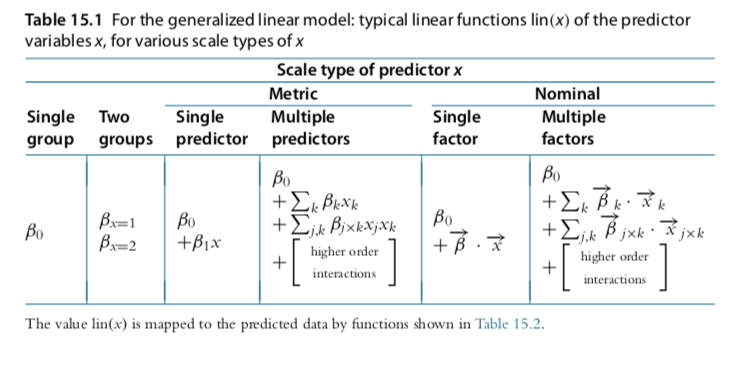
\includegraphics[width=0.8\textwidth]{linear_functions}
        \caption{Typical linear functions}
        \label{fig:linear_functions}
    \end{figure}
\end{itemize}
\end{document}
